\documentclass[xcolor=table, 10pt, aspectratio=43]{beamer}

%\usepackage{arev}
\usepackage{amsmath,amssymb,amscd}
\usepackage{dsfont}
\usepackage{mathrsfs}
\usepackage{yfonts}
\usepackage{bm}
\usepackage{graphicx}
\usepackage{tabularx}
\usepackage{animate}
%\usepackage{mathtools}
%\usepackage{ifthen}

%\usepackage{xeCJK}
%\usepackage{fontspec}
%\newfontfamily\cjkfont{PingFang SC}
%\setCJKmainfont{PingFang SC}
\newcolumntype{x}{>{\centering\arraybackslash}X}
\renewcommand{\arraystretch}{1.5}
\newcommand{\uone}{\mathrm U(1)}

\usepackage{tikz}
	\usetikzlibrary{calc}
	\usetikzlibrary{arrows,shapes, positioning, matrix}
	\usetikzlibrary{decorations.markings}
	\tikzset{>=stealth}
	\tikzstyle arrowstyle=[scale=1]
	\tikzstyle directed=[postaction={decorate,decoration={markings,
 	   mark=at position .15 with {\arrow[arrowstyle]{stealth}}}}]
\tikzstyle string=[thick,postaction={decorate,decoration={markings,
    mark=at position .55 with {\arrow[arrowstyle]{stealth}}}}]
\tikzstyle dual_string=[dashed,postaction={decorate,decoration={markings,
    mark=at position .55 with {\arrow[arrowstyle]{stealth}}}}]

\tikzstyle dw=[thick,postaction={decorate,decoration={markings,
    mark=at position 1 with {\arrow[arrowstyle]{stealth}}}}]
\tikzstyle group=[mbg]
\newcommand*{\halfway}{0.5*\pgfdecoratedpathlength+.5*8pt}\tikzstyle arrowstyle=[scale=1]
\newcommand*{\halfwayb}{0.5*\pgfdecoratedpathlength}
\tikzstyle arrowstyle=[scale=1]
\tikzstyle fermion=[thick,postaction={decorate},decoration={markings,
    mark=at position \halfway with {\arrow[arrowstyle]{latex}}}]
\tikzstyle fermion2=[thick,postaction={decorate},decoration={markings,
        mark=at position \halfwayb with {\arrow[arrowstyle]{latex}}}]

\usepackage{pgffor}
\newcommand{\mb}[1]{\mathbf{#1}}
\renewcommand{\cal}[1]{\mathcal{#1}}

\newcommand{\ag}[2]{#1_\mb{#2}}
\newcommand{\cohosub}[1]{\scalebox{0.72}{\textswab{#1}}}
\newcommand{\cohosubsub}[1]{\scalebox{0.6}{\textswab{#1}}}
\newcommand{\coho}[1]{\textswab{#1}}

\DeclareMathOperator{\tr}{Tr}
\DeclareMathOperator{\im}{Im}
\DeclareMathOperator{\re}{Re}

\mode<presentation>
{
  %\usetheme{Warsaw}
  % or ...
  %\useoutertheme{rectangle}
  \setbeamertemplate{frametitle}[default][center]
  \defbeamertemplate{itemize item}{flat}{\begin{pgfpicture}{-1ex}{0ex}{1ex}{2ex}
      \pgfpathcircle{\pgfpoint{0pt}{.6ex}}{0.6ex}
      \pgfusepath{fill}
    \end{pgfpicture}%
  }
  \defbeamertemplate{itemize subitem}{flat}{\footnotesize\raise0.5pt\hbox{\textbullet}}
  \defbeamertemplate{itemize subsubitem}{flat}{\footnotesize\raise0.5pt\hbox{\textbullet}}

  %\useinnertheme{circles}
  \setbeamertemplate{items}[flat]
  \setbeamertemplate{sections/subsections in toc}[circle]
  \setbeamertemplate{blocks}[rounded]
  \setbeamertemplate{title page}[default][colsep=-4bp,rounded=true]
  \setbeamertemplate{part page}[default][colsep=-4bp,rounded=true]
  \setbeamercovered{transparent}
  %\usecolortheme{spruce}
  %\definecolor{THU}{RGB}{116,61,130}
  \definecolor{mbg}{RGB}{0,0,160}
  \setbeamercolor*{palette primary}{fg=white,bg=mbg}
  \setbeamercolor*{titlelike}{parent=palette primary}
  \setbeamercolor*{structure}{fg=mbg}
  \setbeamercolor{frametitle}{fg=white,bg=mbg}
  % or whatever (possibly just delete it)
  \setbeamercolor{block title}{bg=mbg,fg=white}
  \setbeamercolor{block body}{bg=mbg!15}


  \addtobeamertemplate{navigation symbols}{}{ \hspace{1em}%
    \usebeamerfont{footline}%
    \insertframenumber / \inserttotalframenumber }
}


%\usepackage[english]{babel}
% or whatever

%\usepackage[latin1]{inputenc}
% or whatever

%\usepackage{times}
%\usepackage[T1]{fontenc}
% Or whatever. Note that the encoding and the font should match. If T1
% does not look nice, try deleting the line with the fontenc.

\title[Space-group SPTs] % (optional, use only with long paper titles)
{Real-Space Classification of Bosonic Space-Group SPTs}

\author[Y Qi] % (optional, use only with lots of authors)
{Yang~Qi}
% - Give the names in the same order as the appear in the paper.
% - Use the \inst{?} command only if the authors have different
%   affiliation.

\institute[Fudan] % (optional, but mostly needed)
{Department of Physics, Fudan University}
% - Use the \inst command only if there are several affiliations.
% - Keep it simple, no one is interested in your street address.

%\date{2016 Annual Meeting of Fudan CFTPP} % (optional, should be abbreviation of conference name)
%{Fudan University, Oct 13 2015}
\date{MIT, Aug. 20 2018}
% - Either use conference name or its abbreviation.
% - Not really informative to the audience, more for people (including
%   yourself) who are reading the slides online

\subject{Theoretical Physics}
% This is only inserted into the PDF information catalog. Can be left
% out.



% If you have a file called "university-logo-filename.xxx", where xxx
% is a graphic format that can be processed by latex or pdflatex,
% resp., then you can add a logo as follows:

\pgfdeclareimage[height=1cm]{university-logo}{../resources/fudan}
\logo{\pgfuseimage{university-logo}}

\AtBeginSection[]
{
  \begin{frame}<beamer>{Outline}
			\tableofcontents[currentsection,currentsubsection]
  \end{frame}
}


% Delete this, if you do not want the table of contents to pop up at
% the beginning of each subsection:

\begin{document}

\begin{frame}
  \titlepage
\end{frame}

\begin{frame}{References}
\begin{itemize}
\item Zhi-Da Song: Institute of Physics, Beijing $\Rightarrow$ Princeton.
\item Chen Fang: Institute of Physics, Beijing.
\begin{center}
	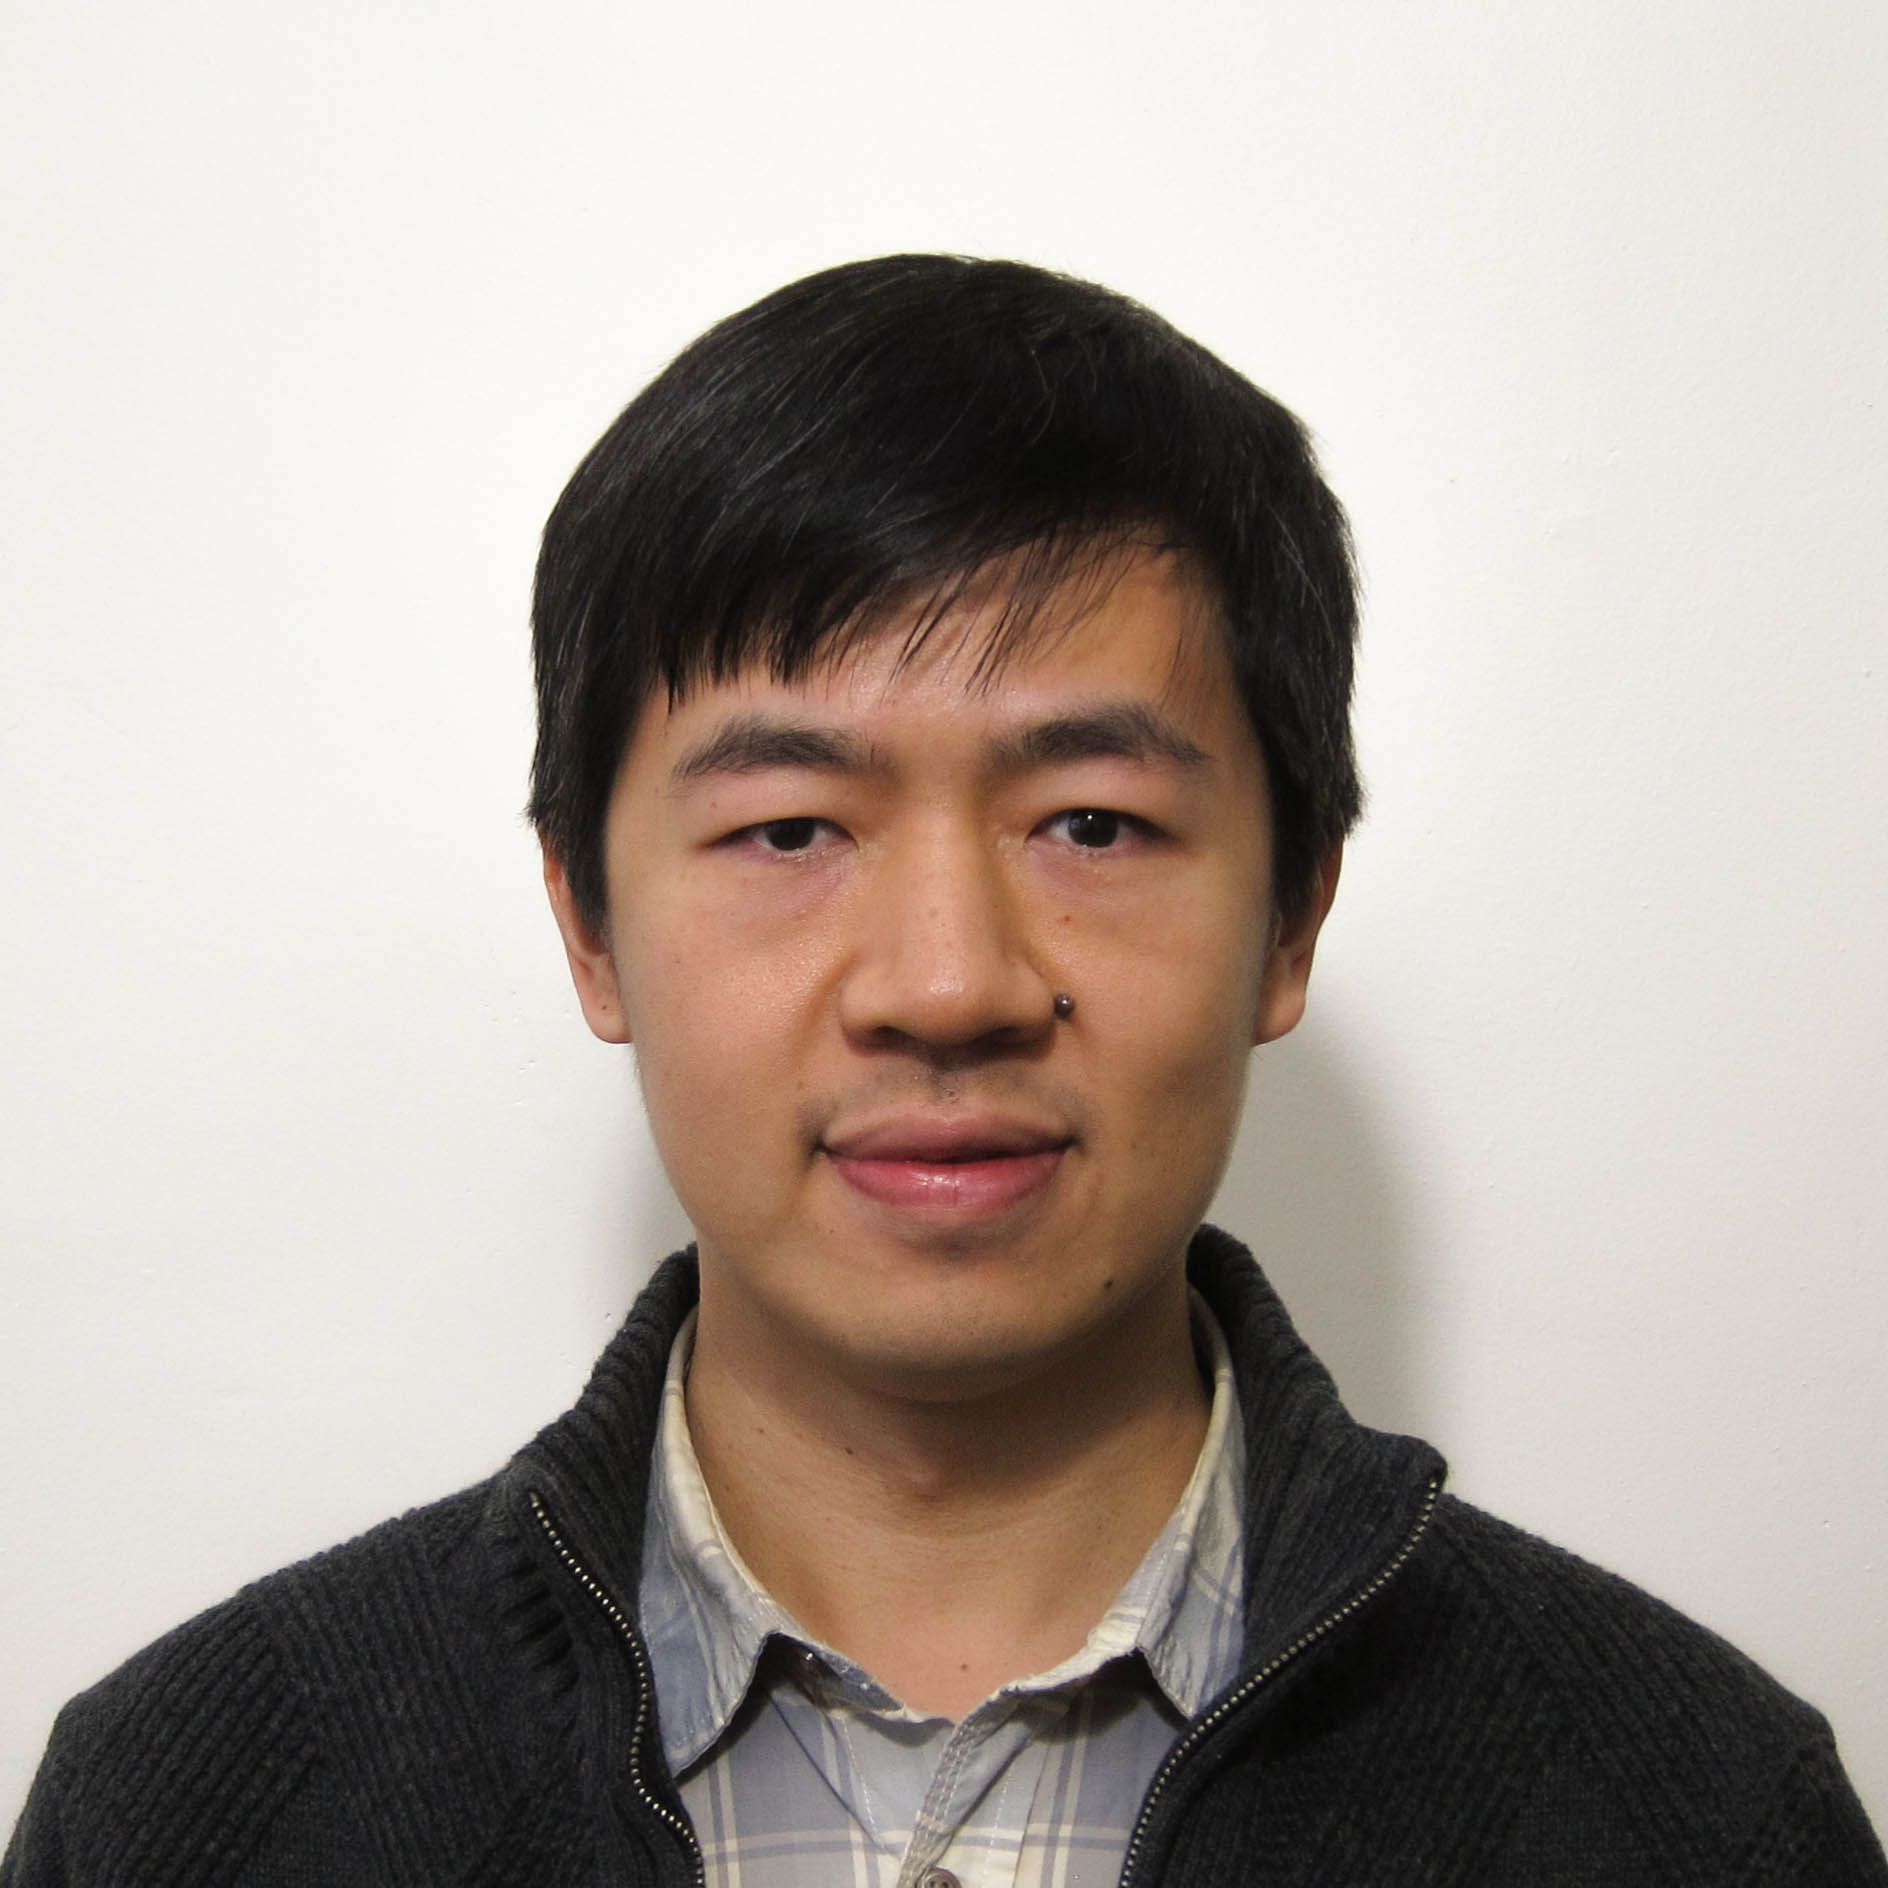
\includegraphics[height=3cm]{../people/chenfang}
\end{center}
\item Working in progress.
\end{itemize}
\end{frame}

\section{Introduction to Symmetry-Protected Topological (SPT) states}

\begin{frame}
  \frametitle{Symmetry-Protected Topological (SPT) states}
\end{frame}

\begin{frame}
  \frametitle{SPT states of onsite symmetry}
  \begin{itemize}
    \item Classification is given by group cohomology
    \[H^{d+1}[G, \uone_T].\]
		\item Symmetric cocycles:
		\[\omega(gg_0,\ldots gg_{d+1})=\rho_T(g)\omega(g_0,\ldots g_{d+1}).\]
		\item Bulk-boundary correspondence:
		\[d\omega = \nu,\quad d:H^d[G, \uone_T]\rightarrow H^{d+1}[G, \uone_T]\]
		\[d\omega(g_0,\ldots,g_{d+1})
		=\sum_i(-1)^i\omega(g_0,\ldots,\hat g_i,\ldots,g_{d+1}).\]
\begin{center}
	\begin{tikzpicture}
	\fill (.5, .5)--(4.5, 0.5)--(5, 1)--(5, 2)--(1, 2)--(0.5, 1.5)--(0.5, 0.5) [mbg!15];
	\node at (2.75, 1.5) {$\nu$};
	\fill (0.5, 0.5)--(4.5, 0.5)--(5, 1)--(1, 1)--(0.5, 0.5) [mbg];
	\node  [text=white] at (2.75, 0.75) {$\omega$};
	\draw (1, 1)--(1, 2) [black!40];
	\draw (0.5, 0.5)--(0.5, 1.5) [black!40];
	\draw (5, 1)--(5, 2) [black!40];
	\end{tikzpicture}
\end{center}
  \end{itemize}
\end{frame}
\section{Space-group SPTs: dimensional reduction}
\section{Building an SPT from building blocks}
\begin{frame}
	\frametitle{Space-group SPTs are made of building blocks}
	\begin{columns}
		\column{.4\textwidth}
		\begin{center}
			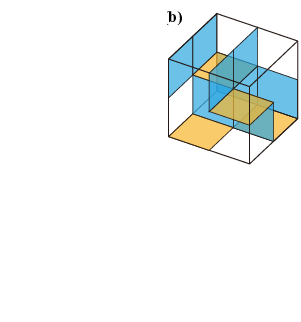
\includegraphics[width=\textwidth]{blocks}
		\end{center}
		\column{.6\textwidth}
		\begin{itemize}
			\item We divide the space into cells compatible with the space-group symmetry.
			\item Decorate 3d SPT on 3-cells; 2d SPT on 2-cells; 1d SPT on 1-cells; 0d SPT on 0-cells;
			\item On a $p$-cell $\sigma$, the SPT state is protected only by $G_\sigma$.
			\[\omega_\sigma\in C^{p+1}[G_\sigma,\uone_T].\]
			\item $G_\sigma$ acts as onsite symmetries.
		\end{itemize}
	\end{columns}
\end{frame}

\begin{frame}
	\frametitle{Decomposition of the space}
	We divide the space into finer cells such that
	\begin{enumerate}
		\item A cell $\sigma$ is maped to one single cell $\sigma^\prime$ under $SG$-action.
		\item $G_\sigma$ acts on $\sigma$ as onsite symmetry.
	\end{enumerate}
	\begin{center}
		\begin{tikzpicture}
			\draw (-2, -2)--(-2, 2)--(2, 2)--(2, -2)--(-2, -2);
			\draw [thick] (0, -2)--(0, 2);
			\filldraw (0, 0) circle (1pt) node [right] {$C_2$};
			\node at (0, -1) [right] {$\tau_1$};
			\node at (0, 1) [left] {$\tau_2$};
			\node at (-1, 0) {$\sigma_1$};
			\node at (1, 0) {$\sigma_2$};
		\end{tikzpicture}
	\end{center}
\end{frame}

\begin{frame}
	\frametitle{A building block}
	\begin{columns}
		\column{.4\textwidth}
		\begin{center}
			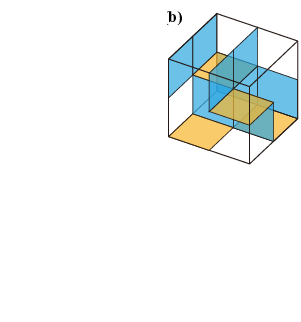
\includegraphics[width=\textwidth]{blocks}
		\end{center}
		\column{.6\textwidth}
		\begin{itemize}
			\item A building block $\hat\omega$ is a collection of cochains:
			\[\hat\omega(\sigma) \in C^{p+1}[G_\sigma, \uone_T].\]
			\item $\hat\omega$ needs to be symmetric under $SG$.
			\item $\hat\omega$ needs to satisfy the bulk-boundary relation:
			\[d\hat\omega(\tau) = \sum_{\sigma:\tau\in\partial\sigma}\hat\omega(\sigma).\]
			\item Need to find when two blocks can be deformed to each other: $\hat\omega\simeq\hat\omega^\prime$.
		\end{itemize}
	\end{columns}
\end{frame}

\begin{frame}
	\frametitle{Symmetric conditions}
	\begin{columns}
		\column{.4\textwidth}
		\begin{tikzpicture}
			\draw (0, 0)--(2, 0)--(2, 2)--(0, 2)--(0, 0);
			\draw (2, 4)--(4, 4)--(4, 6)--(2, 6)--(2, 4);
			\draw [thick,->] (1, 1) node [below] {$\hat\omega(\sigma$)} --
			(3, 5) node [above] {$\hat\omega(\sigma^\prime)$};
			\node at (2, 3) [right] {$g$};
		\end{tikzpicture}
		\column{.6\textwidth}
		\begin{itemize}
			\item If $g:\sigma\rightarrow\sigma^\prime$, then the cochains attached must be ``identical''.
			\item $G_\sigma\neq G_{\sigma'}$, but they are isomorphic:
			\[G_{\sigma'}=gG_\sigma g^{-1}\simeq G_\sigma.\]
			\item This induces another isomorphism between the cochain spaces:
			\[C^{p+1}[G_{\sigma'},\uone_T]\simeq C^{p+1}[G_\sigma,\uone_T]\]
			\item $\hat\omega(\sigma)$ and $\hat\omega(\sigma')$ are related by this isomorphism, which we denote by
			\[\hat\omega(\sigma') = g\cdot \hat\omega(\sigma).\]
			\item Only decorations on symmetry-unrelated cells are independent: finite \# of them.
		\end{itemize}
	\end{columns}
\end{frame}

\begin{frame}
	\frametitle{Bulk-boundary relations}
	\begin{columns}
		\column{.58\textwidth}
		\begin{itemize}
			\item Naively:
			\[d\hat\omega(\tau) = \hat\omega(\sigma_1)
			+\hat\omega(\sigma_2)+\hat\omega(\sigma_3)+\hat\omega(\sigma_4)\]
			\item A subtlety: $\tau$ has more symmetry operations than $\sigma$: $G_\tau \supseteq G_\sigma$
			\item Hence, $\hat\omega(\sigma_i)$ is not $G_\tau$-symmetric.
			\item When $[G_\tau:G_\sigma]>1$: $\tau$ borders $[G_\tau:G_\sigma]$ symmetry-related copies of $\sigma_i$.
			\item $\hat\omega(\sigma_1)
			+\hat\omega(\sigma_2)+\hat\omega(\sigma_3)+\hat\omega(\sigma_4)\in C^{p+1}[G_\tau,\uone_T]$.
			\item We can define a boundary-transfer operation $\partial\hat\omega$:
			\[(\partial\hat\omega)(\tau)=\hat\omega(\sigma_1)
			+\hat\omega(\sigma_2)+\hat\omega(\sigma_3)+\hat\omega(\sigma_4).\]
			\item Cocycle equation: $d\hat\omega - \partial\hat\omega=0.$
		\end{itemize}
		\column{.42\textwidth}
		\begin{tikzpicture}
			\draw (0, 1)--(-1, 1)--(-2, 0)--(2, 0)--(3, 1)--(1, 1);
			\draw [thick] (0, 0)--(1, 1);
			\node at (.5, .5) [above] {$\tau$};
			\draw (1, 1)--(1, 3)--(0, 2)--(0, -2)--(0, -2)--(1, -1)--(1, 0);
			\node at (.5, 1.5) {$\sigma_1$};
			\node at (1.5, .5) {$\sigma_2$};
			\node at (.5, -0.5) {$\sigma_3$};
			\node at (-0.5, .5) {$\sigma_4$};
		\end{tikzpicture}
	\end{columns}
\end{frame}

\begin{frame}
	\frame{Coboundary equivalence}
\end{frame}
\section{Mathematical details}
\section{Conclusion}


\end{document}
